% Title: glps_renderer figure
% Creator: GL2PS 1.3.8, (C) 1999-2012 C. Geuzaine
% For: Octave
% CreationDate: Mon Nov 23 09:01:15 2015
\setlength{\unitlength}{1pt}
\begin{picture}(0,0)
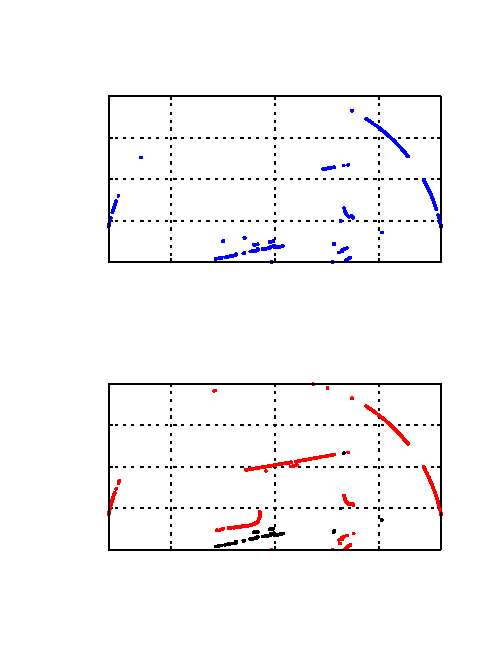
\includegraphics{fig/bg_process-inc}
\end{picture}%
\begin{picture}(225,300)(0,0)
\fontsize{8}{0}
\selectfont\put(74.1421,177.04){\makebox(0,0)[t]{\textcolor[rgb]{0,0,0}{{-5000}}}}
\fontsize{8}{0}
\selectfont\put(123.943,177.04){\makebox(0,0)[t]{\textcolor[rgb]{0,0,0}{{0}}}}
\fontsize{8}{0}
\selectfont\put(173.744,177.04){\makebox(0,0)[t]{\textcolor[rgb]{0,0,0}{{5000}}}}
\fontsize{8}{0}
\selectfont\put(39.25,182.02){\makebox(0,0)[r]{\textcolor[rgb]{0,0,0}{{0}}}}
\fontsize{8}{0}
\selectfont\put(39.25,201.941){\makebox(0,0)[r]{\textcolor[rgb]{0,0,0}{{2000}}}}
\fontsize{8}{0}
\selectfont\put(39.25,221.861){\makebox(0,0)[r]{\textcolor[rgb]{0,0,0}{{4000}}}}
\fontsize{8}{0}
\selectfont\put(39.25,241.782){\makebox(0,0)[r]{\textcolor[rgb]{0,0,0}{{6000}}}}
\fontsize{8}{0}
\selectfont\put(39.25,261.702){\makebox(0,0)[r]{\textcolor[rgb]{0,0,0}{{8000}}}}
\fontsize{8}{0}
\selectfont\put(123.943,271.702){\makebox(0,0)[b]{\textcolor[rgb]{0,0,0}{{Raw laser data}}}}
\fontsize{8}{0}
\selectfont\put(74.1421,39.0403){\makebox(0,0)[t]{\textcolor[rgb]{0,0,0}{{-5000}}}}
\fontsize{8}{0}
\selectfont\put(123.943,39.0403){\makebox(0,0)[t]{\textcolor[rgb]{0,0,0}{{0}}}}
\fontsize{8}{0}
\selectfont\put(173.744,39.0403){\makebox(0,0)[t]{\textcolor[rgb]{0,0,0}{{5000}}}}
\fontsize{8}{0}
\selectfont\put(39.25,44.0204){\makebox(0,0)[r]{\textcolor[rgb]{0,0,0}{{0}}}}
\fontsize{8}{0}
\selectfont\put(39.25,63.9408){\makebox(0,0)[r]{\textcolor[rgb]{0,0,0}{{2000}}}}
\fontsize{8}{0}
\selectfont\put(39.25,83.8613){\makebox(0,0)[r]{\textcolor[rgb]{0,0,0}{{4000}}}}
\fontsize{8}{0}
\selectfont\put(39.25,103.782){\makebox(0,0)[r]{\textcolor[rgb]{0,0,0}{{6000}}}}
\fontsize{8}{0}
\selectfont\put(39.25,123.702){\makebox(0,0)[r]{\textcolor[rgb]{0,0,0}{{8000}}}}
\fontsize{8}{0}
\selectfont\put(123.943,133.702){\makebox(0,0)[b]{\textcolor[rgb]{0,0,0}{{Background model and extracted foreground}}}}
\end{picture}
